\documentclass[final,2p]{elsarticle}

\usepackage{amssymb}
\usepackage{amsmath}
\usepackage{hyperref}
\usepackage{tikz}
\usepackage{graphicx}
\usepackage{subfig}
\usepackage{textcomp}
\usetikzlibrary{fit,arrows,calc,positioning}

\journal{Udacity}

\begin{document}

\begin{frontmatter}

\title{Capstone Project}

\author{Martin Pij{\'a}k}

\address{Bratislava, Slovakia}

\begin{abstract}
%% Text of abstract
This is project for using Machine Learning methods in futures trading.
\end{abstract}

\begin{keyword}
Machine Learning \sep{Trading} \sep{Udacity} \sep{Nanodegree}
%% keywords here, in the form: keyword \sep keyword

\end{keyword}

\end{frontmatter}

%%
%% Start line numbering here if you want
%%
%% \linenumbers

%% main text
\section{Domain}

This project investigates possible futures trading strategies on Chicago Mercantile Exchange (CME) and Intercontinental Exchange (ICE) markets with Machine Learning methods. The goal is to find the trading strategy mostly based on the price, Commitment of Traders report (COT) and seasonality pattern. We will compare this trading strategy to commonly used investing approaches as returns of Nasdaq.

Following commodities were investigated:
\begin{itemize}
    \item \href{https://www.cmegroup.com/trading/metals/precious/gold.html}{Gold}
    \item \href{https://www.cmegroup.com/trading/agricultural/grain-and-oilseed/corn.html}{Corn}
    \item \href{https://www.cmegroup.com/trading/agricultural/softs/coffee.html}{Coffee}
\end{itemize}
\clearpage
\section{Datasets and Inputs}
%% \label{S:1}

I used data from \href{https://www.quandl.com/}{Quandl}. Data contains Open, High, Low, Close and volume (OHLCV) and commitment of traders (COT).
Continuous data was generated by taking contract with the highest volume for the trading day. For details please see \textbf{data-preparation.ipynb}.

\begin{figure}[h!]
\centering
\begin{tabular}{ccc}
\subfloat[Gold]{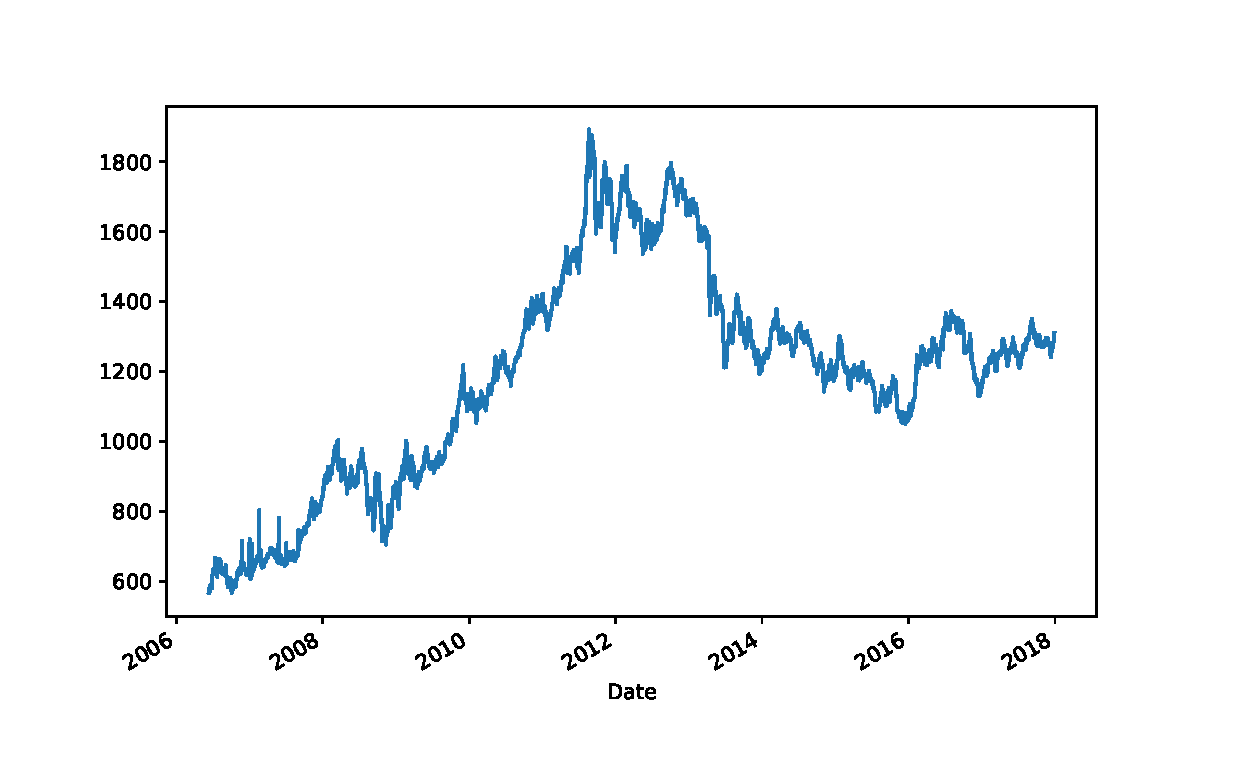
\includegraphics[width = 1.5in]{figures/gold.eps}} &
\subfloat[Corn]{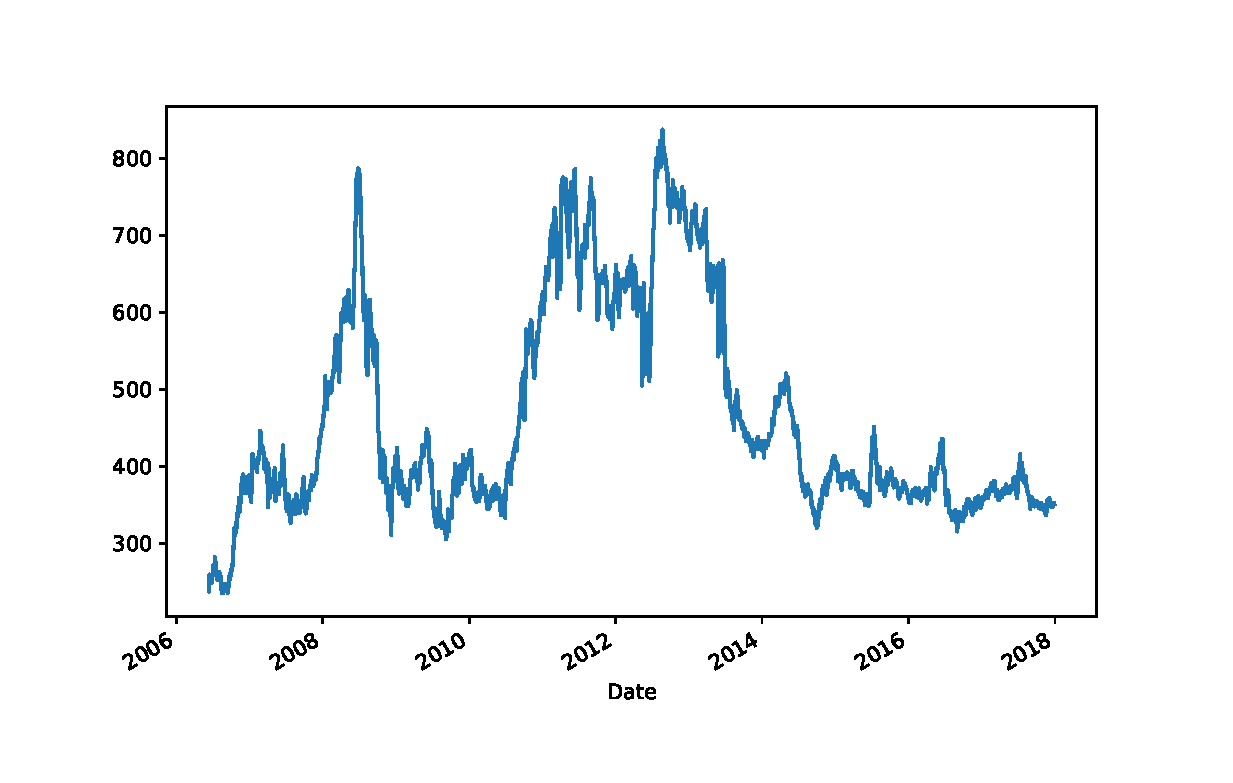
\includegraphics[width = 1.5in]{figures/corn.eps}} &
\subfloat[Coffee]{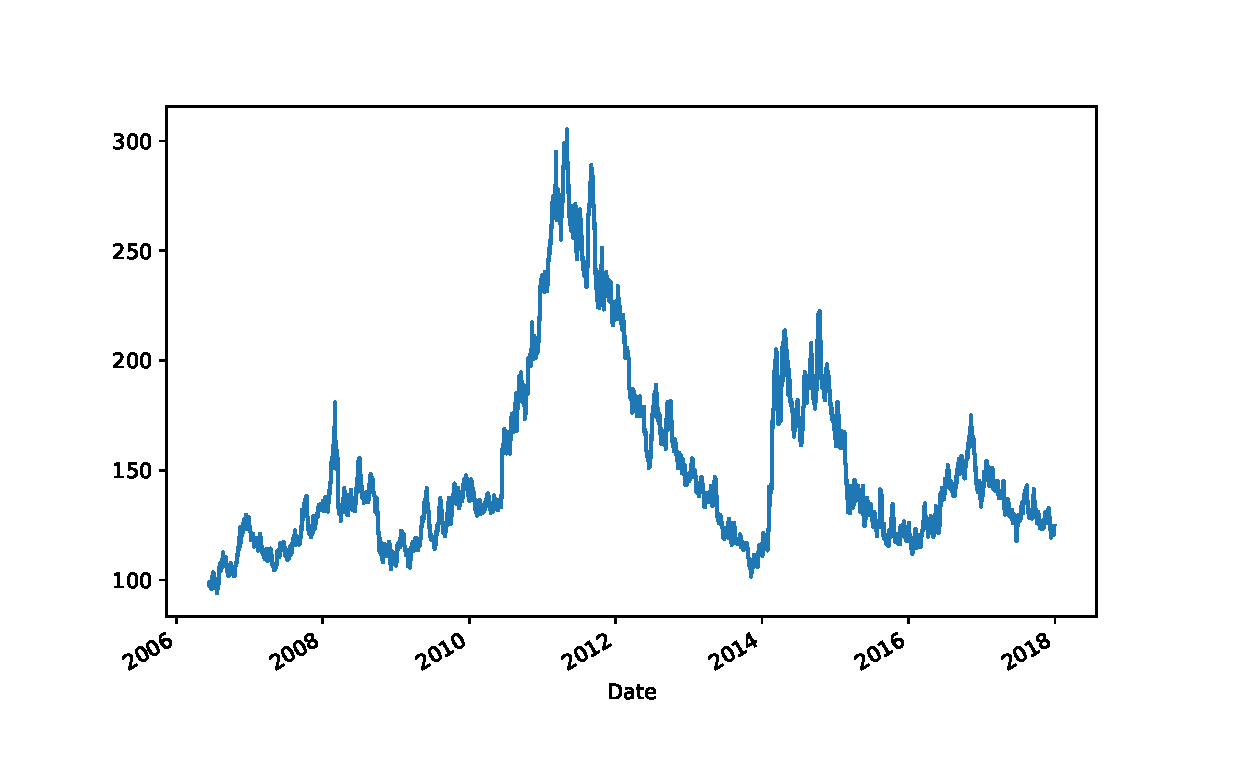
\includegraphics[width = 1.5in]{figures/coffee.eps}}
\end{tabular}
\caption{Close price graphs}
\end{figure}

\section{ML Tools}
Following tools were used:
\begin{itemize}
    \item General ML tools
    \begin{itemize}
        \item \href{https://scikit-learn.org/}{Scikit}
    \end{itemize}
    \item Visualisation
        \begin{itemize}
            \item \href{https://matplotlib.org/}{matplotlib}
            \item \href{https://seaborn.pydata.org/}{seaborn}
        \end{itemize}
    \item Model building tools
        \begin{itemize}
            \item \href{https://keras.io/}{Keras}
            \item \href{https://www.tensorflow.org/}{TensorFlow (keras backend)}
            \item \href{https://www.h2o.ai/}{H2O}
            \item \href{https://lightgbm.readthedocs.io/}{LightGBM}
        \end{itemize}
\end{itemize}

\section{Data analysis}

In the proposal I wanted to investigate classification of volatility. Below is 95\% of daily volatility. 95\% was selected as a simulation of slippage.
General trading idea is to keep trade for a day. 
\begin{figure}[h!]
\centering
\begin{tabular}{ccc}
\subfloat[Gold]{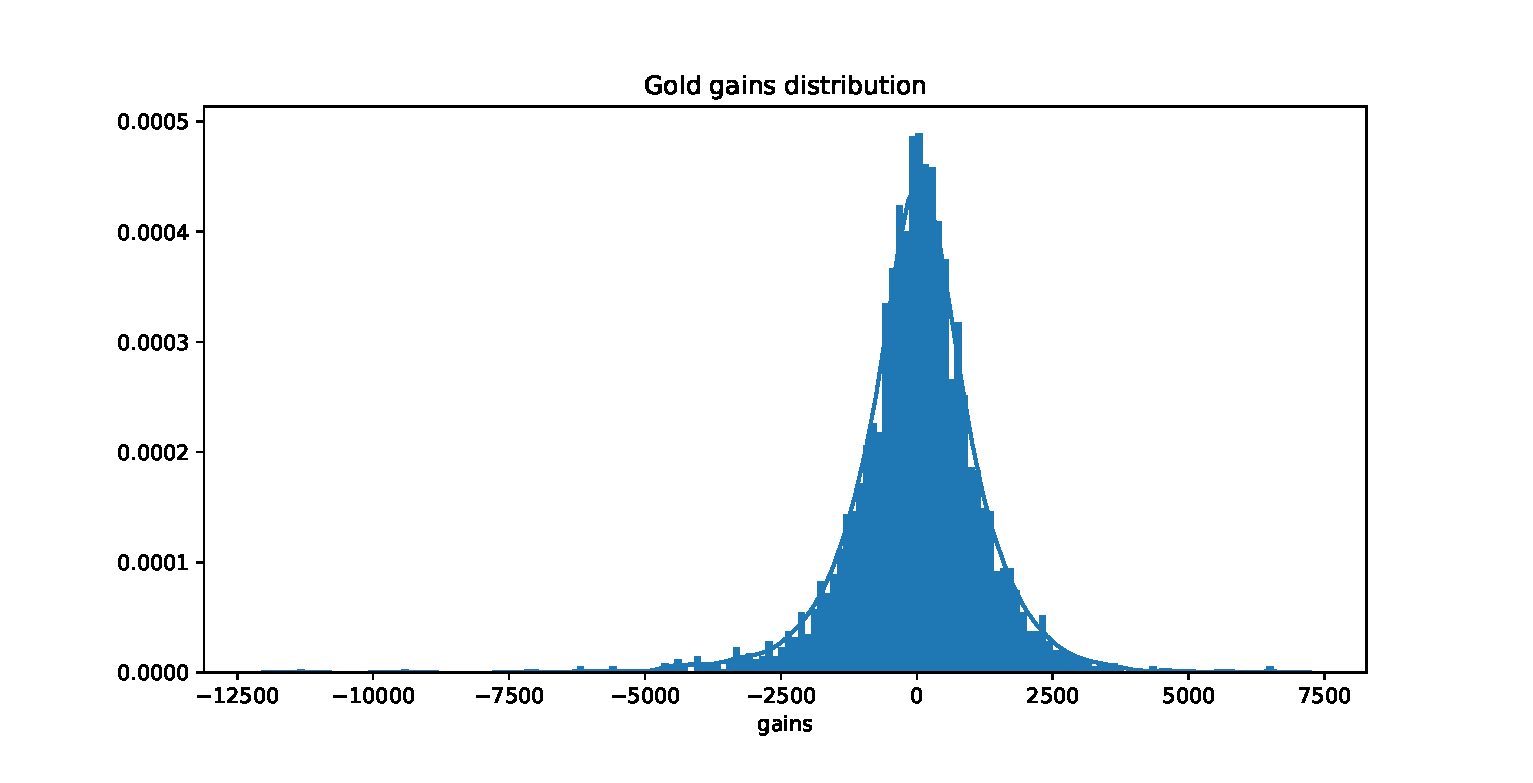
\includegraphics[width = 1.5in]{figures/gold_gains_distribution.eps}} &
\subfloat[Corn]{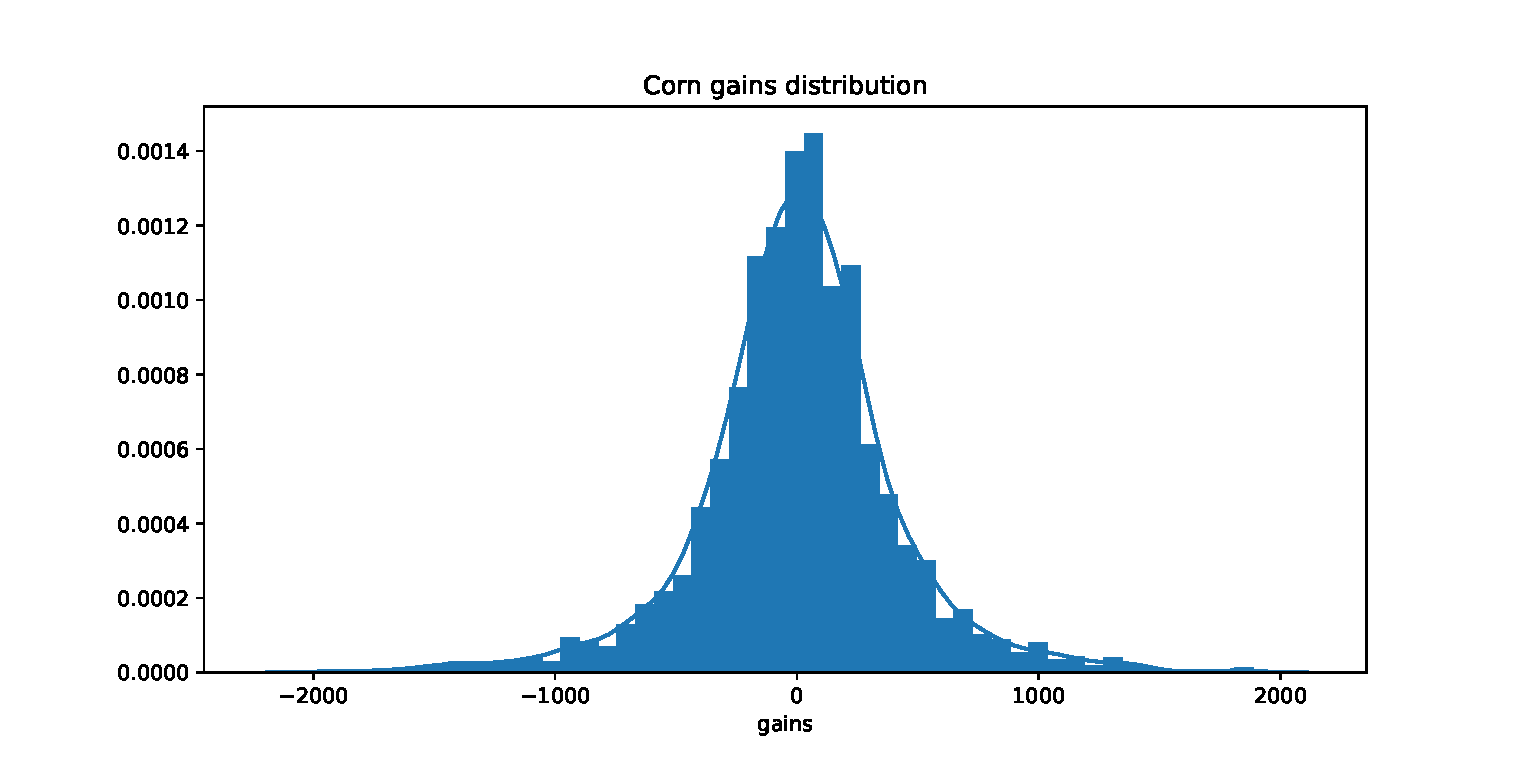
\includegraphics[width = 1.5in]{figures/corn_gains_distribution.eps}} &
\subfloat[Coffee]{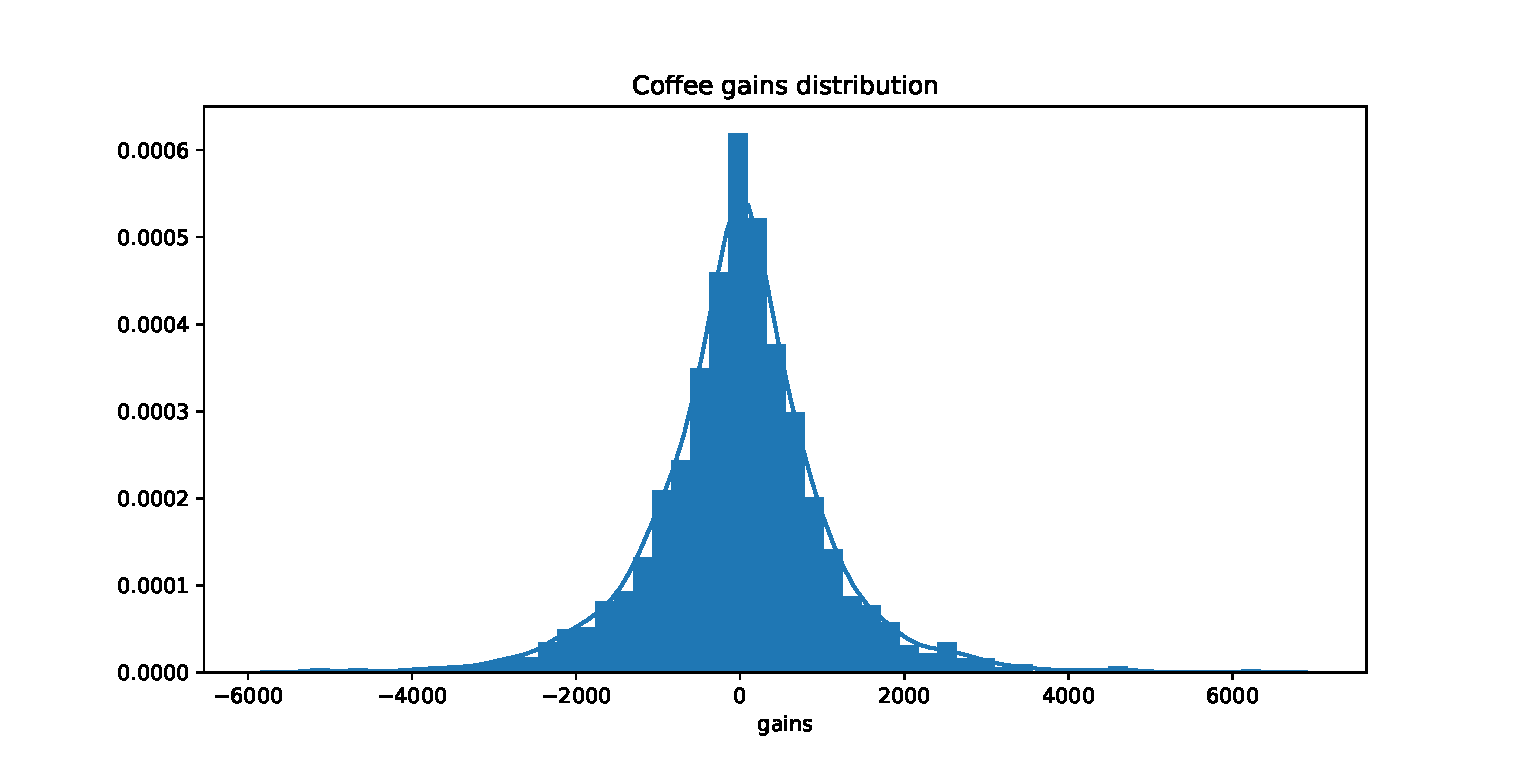
\includegraphics[width = 1.5in]{figures/coffee_gains_distribution.eps}}
\end{tabular}
\caption{Gains distribution}
\end{figure}

Labels were generated based on the trading target.
Target -1 is for short trade. 0 for no trade and 1 for long trade.
\begin{figure}[h!]
\centering
\begin{tabular}{ccc}
\subfloat[Gold]{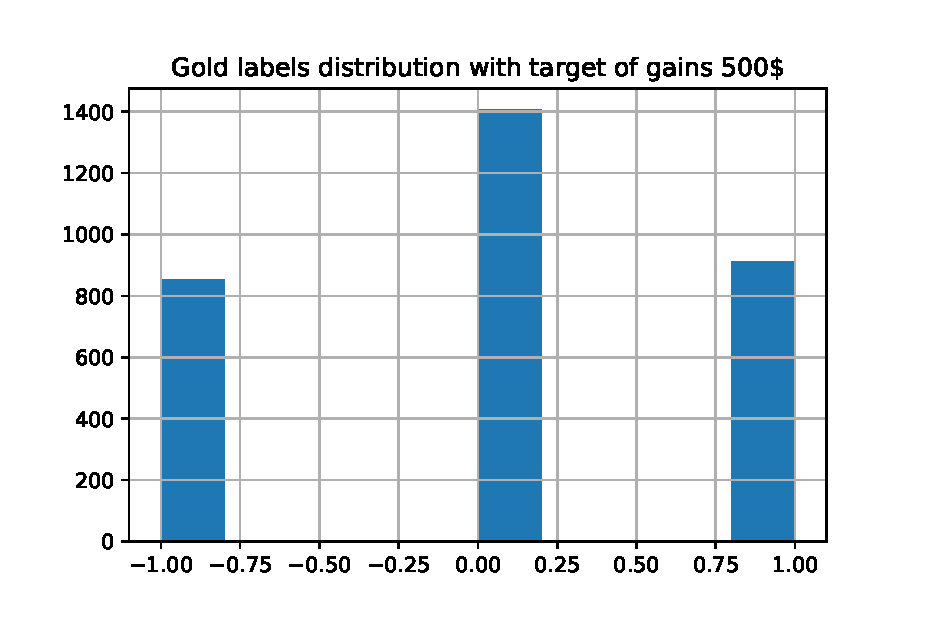
\includegraphics[width = 1.5in]{figures/gold_target_distribution.eps}} &
\subfloat[Corn]{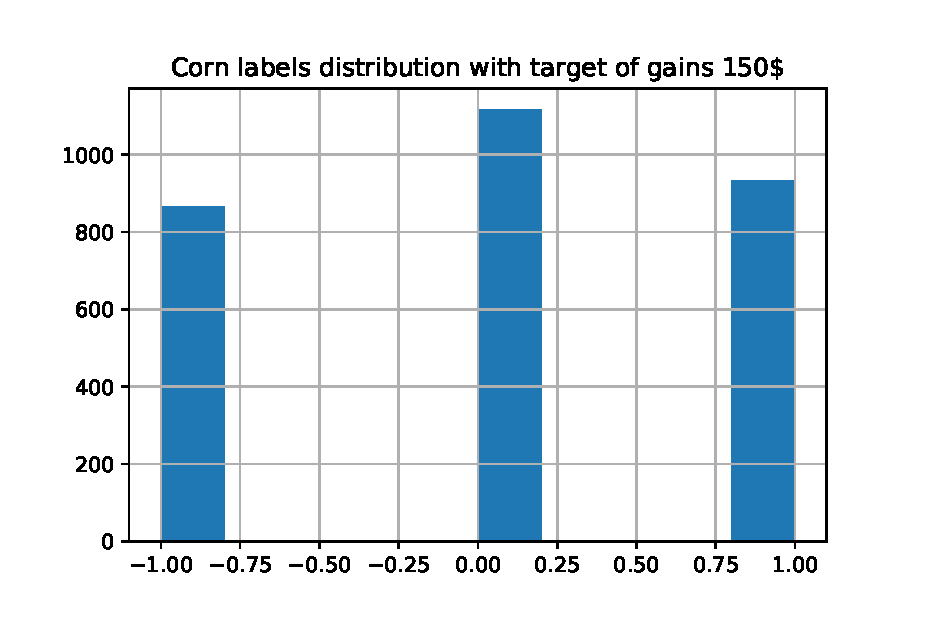
\includegraphics[width = 1.5in]{figures/corn_target_distribution.eps}} &
\subfloat[Coffee]{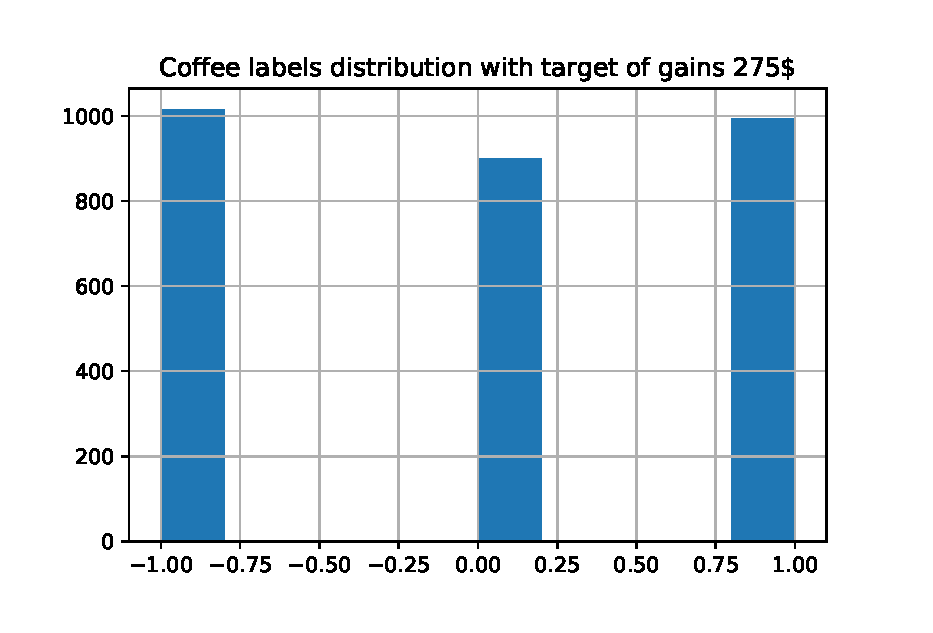
\includegraphics[width = 1.5in]{figures/coffee_target_distribution.eps}}
\end{tabular}
\caption{Labels distribution}
\end{figure}


I decided to have a look at regressor as well.

Based on the past 2 years of trading data (OHLCV and COT) classifier is deciding whether to trade or not.

Approach to training classifier/regressor and evaluation does not take into account that stop-loss can still make trade unsuccessfull.
From Machine Learning perspective the best approach is to have result of classification regression as close to the desired outcome as possible.

Stop-loss was selected so that 90\% of trades will be successfully executed (exited on close).

\begin{figure}[h!]
\centering
\begin{tabular}{cc}
\subfloat[Gold long]{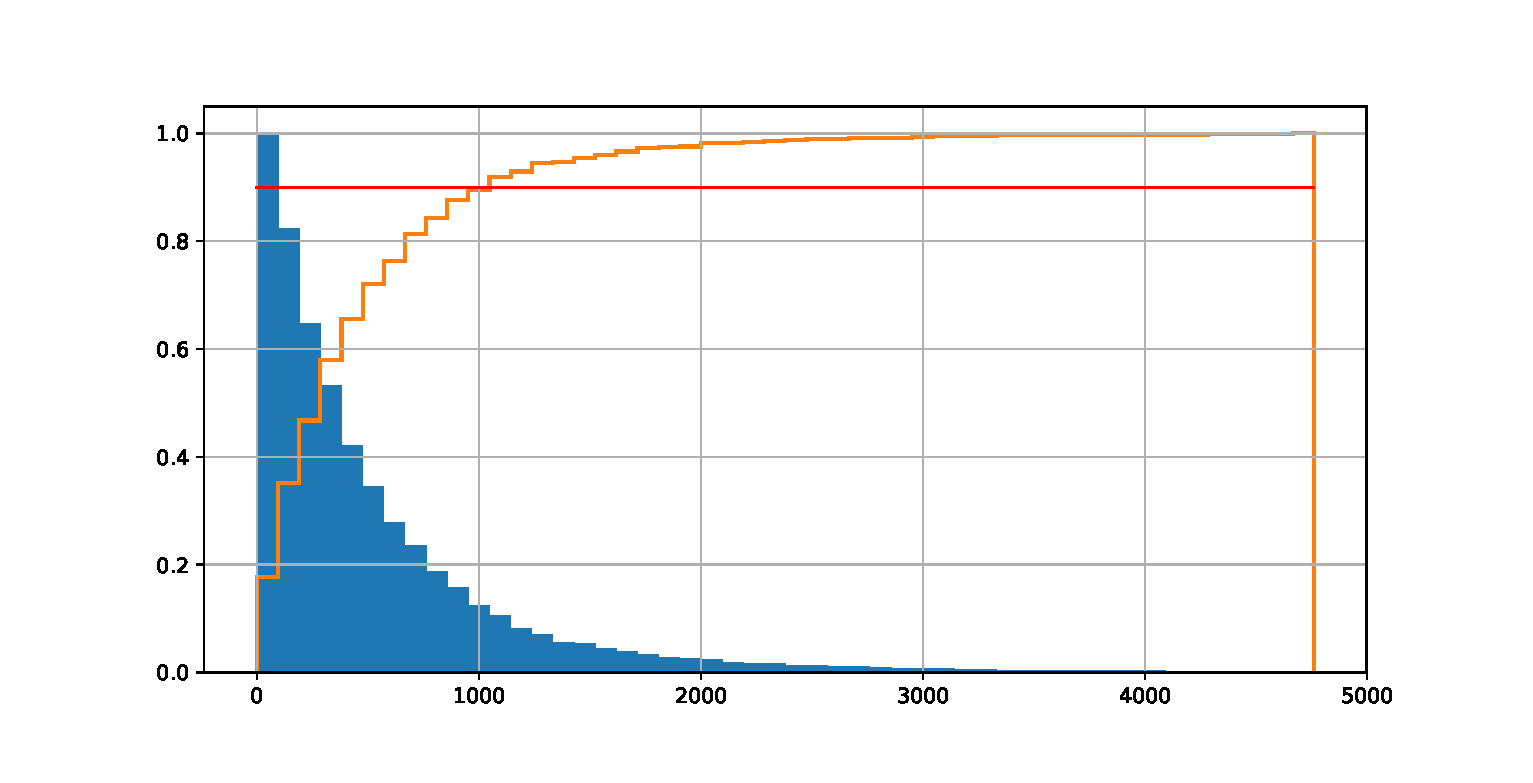
\includegraphics[width = 2in]{figures/gold_stop_loss_long_trades.eps}} &
\subfloat[Gold short]{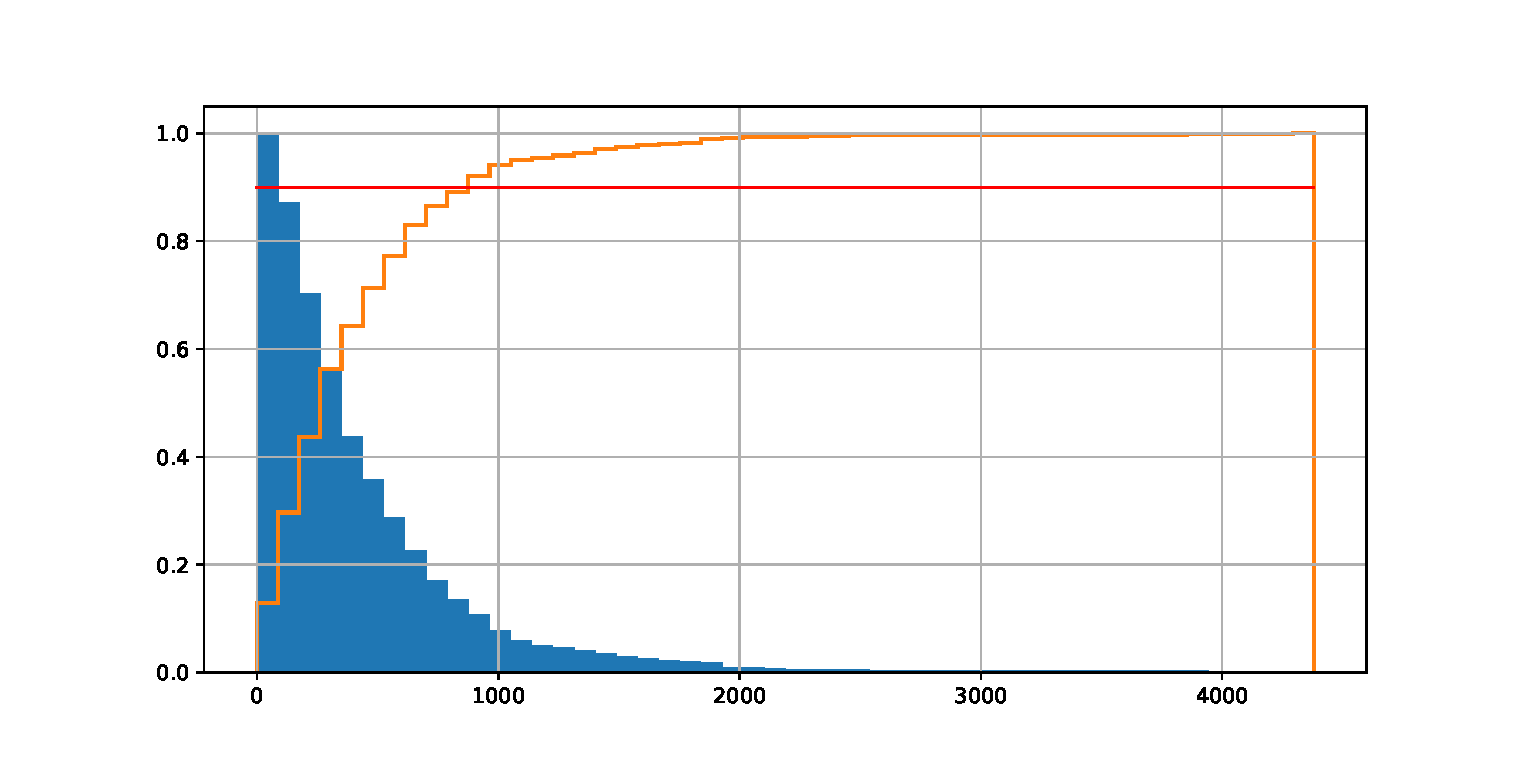
\includegraphics[width = 2in]{figures/gold_stop_loss_short_trades.eps}} \\
\subfloat[Corn long]{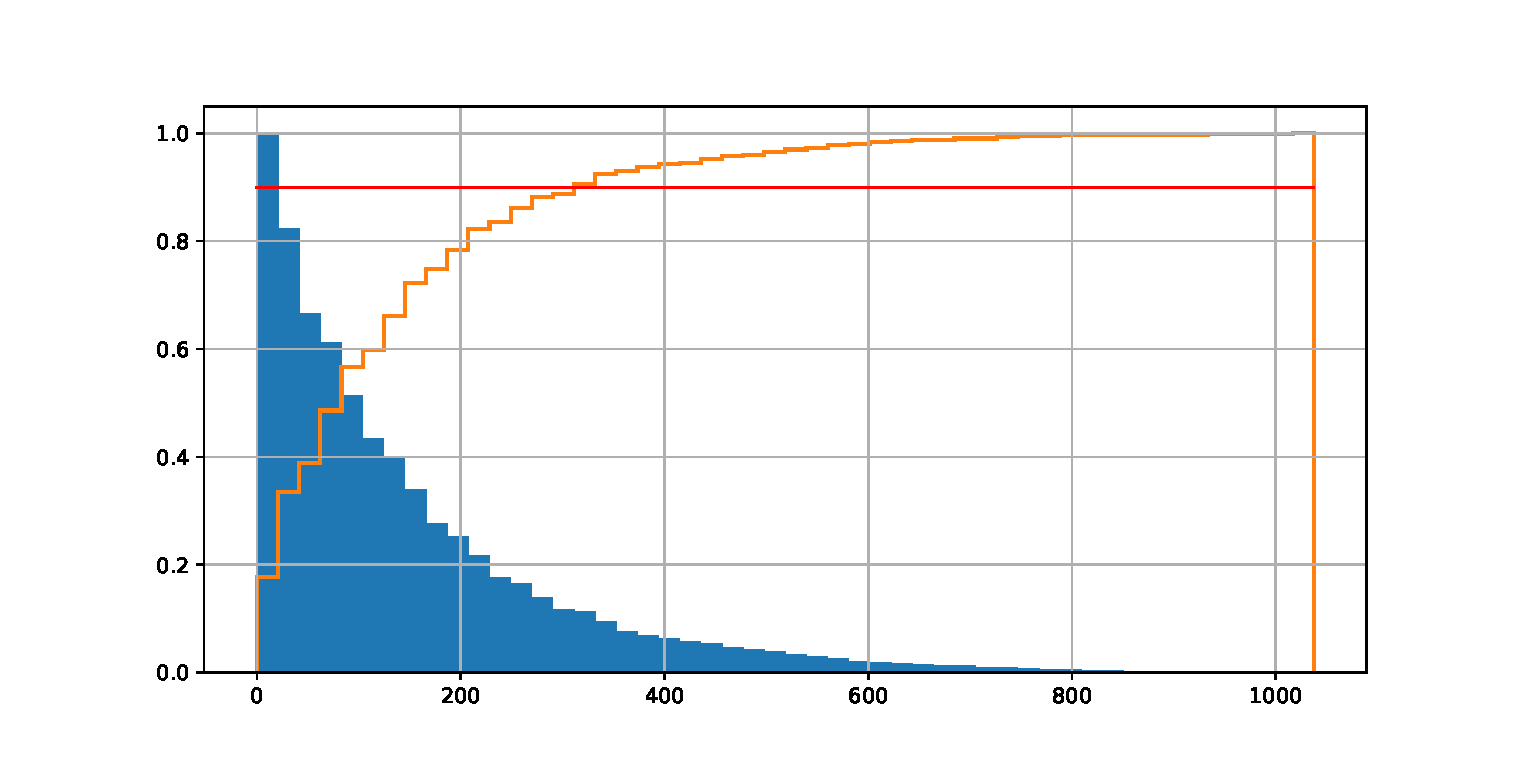
\includegraphics[width = 2in]{figures/corn_stop_loss_long_trades.eps}} &
\subfloat[Corn short]{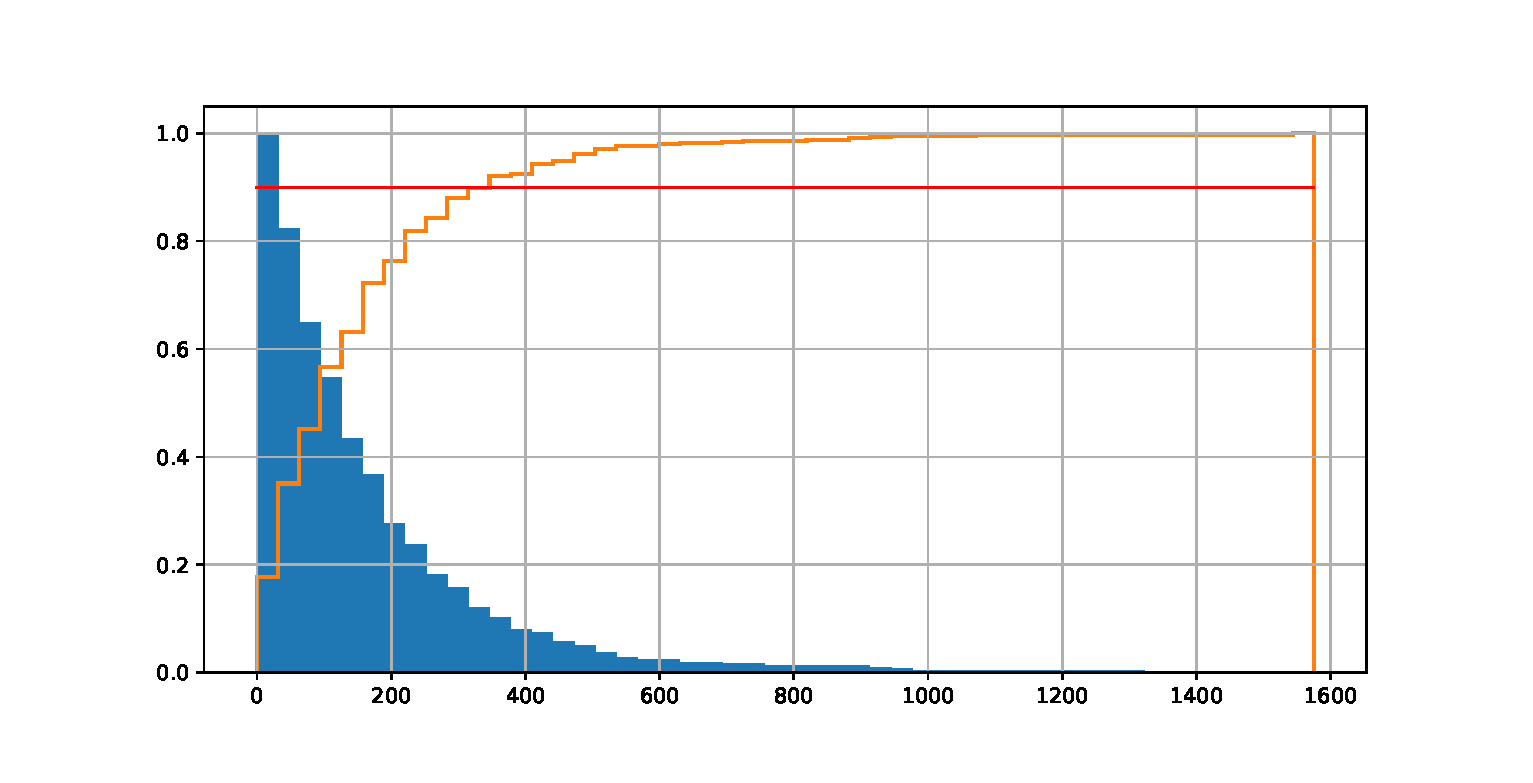
\includegraphics[width = 2in]{figures/corn_stop_loss_short_trades.eps}} \\
\subfloat[Coffee long]{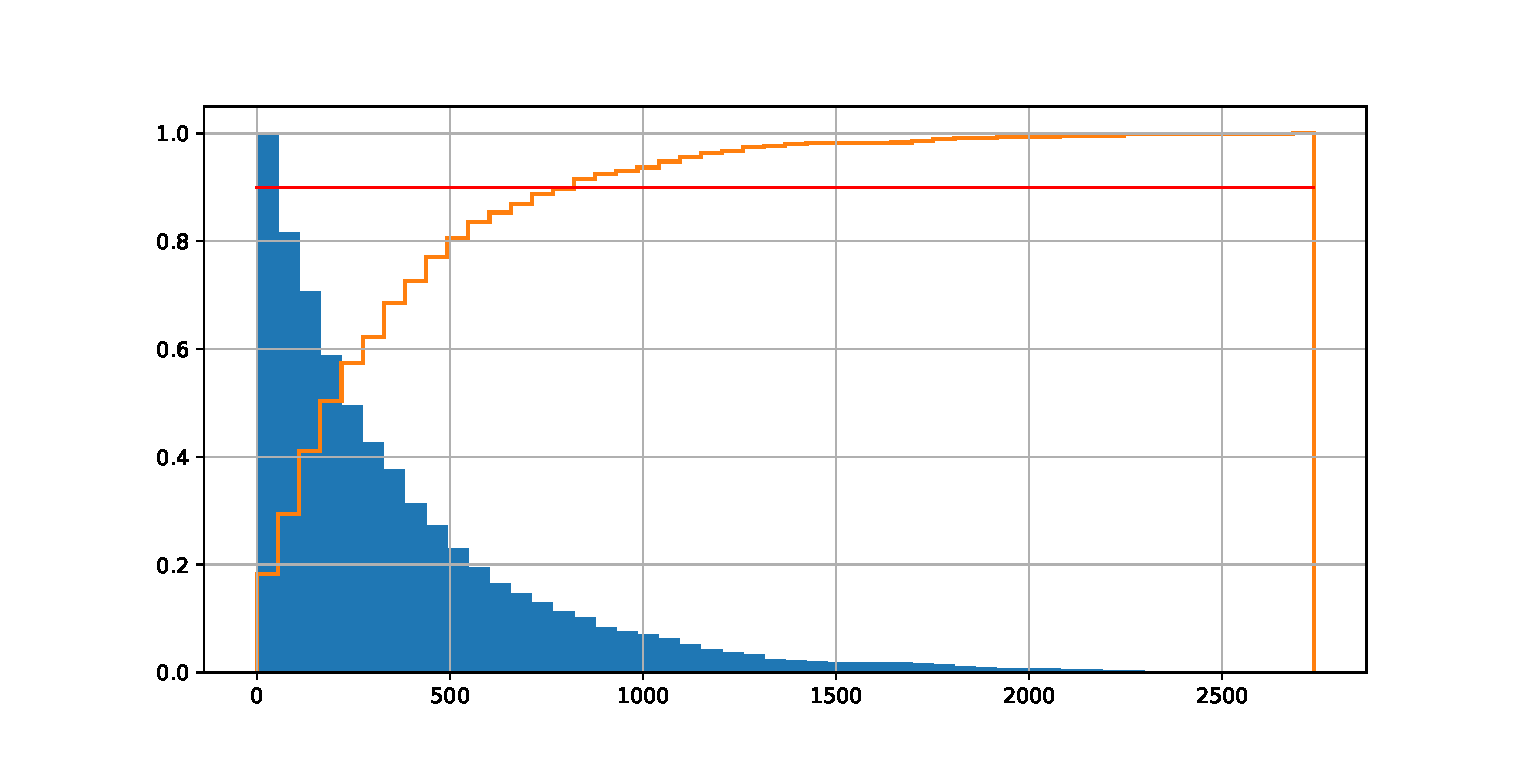
\includegraphics[width = 2in]{figures/coffee_stop_loss_long_trades.eps}} &
\subfloat[Coffee short]{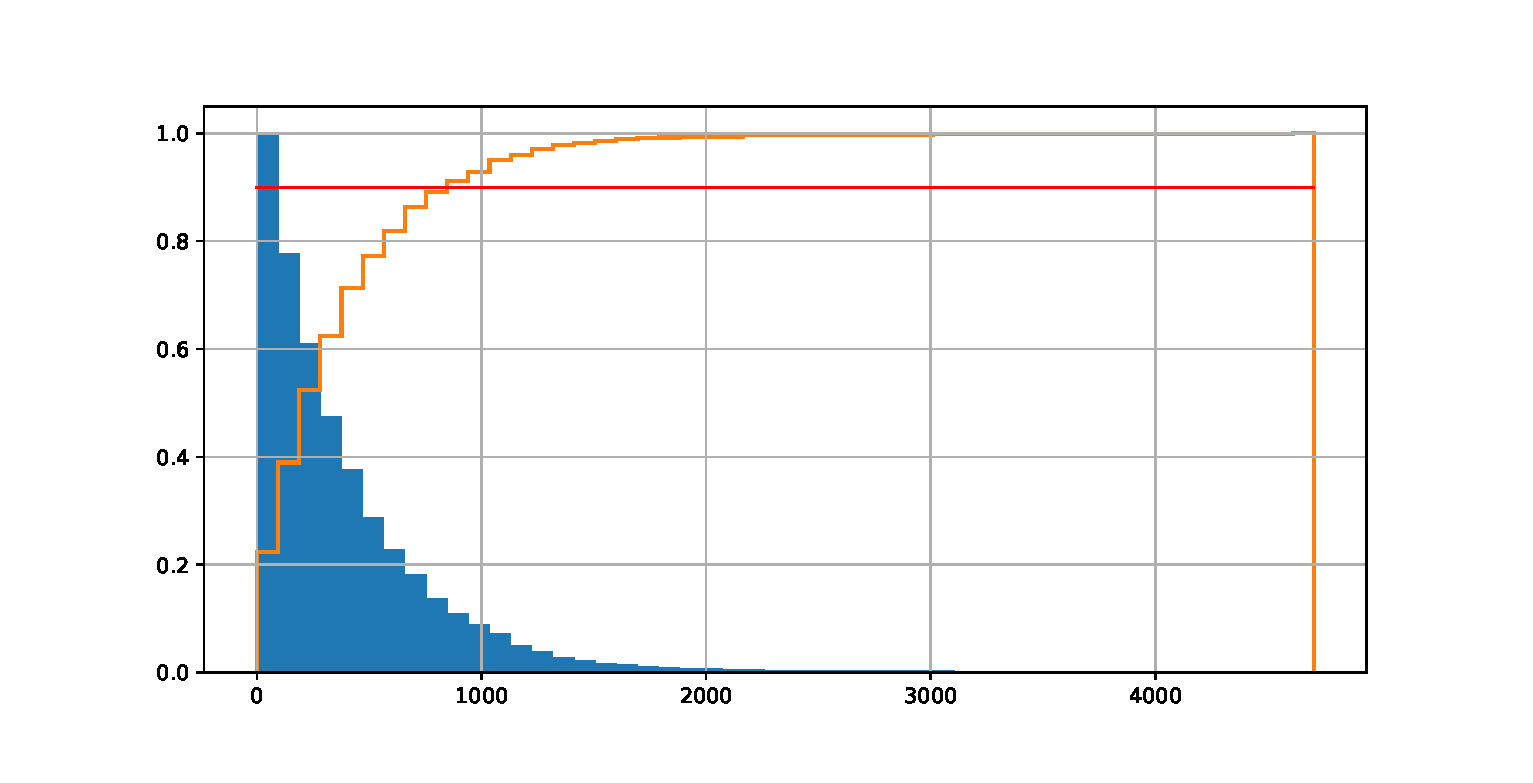
\includegraphics[width = 2in]{figures/coffee_stop_loss_short_trades.eps}}
\end{tabular}
\caption{Stop Loss analysis counter position move}
\end{figure}

\begin{center}
\begin{tabular}{|c|c|c|}
    \hline
    Commodity & Long Stop Loss & Short Stop Loss \\
    \hline
    Gold & 1000 & 800 \\
    Corn & 300 & 300 \\
    Coffee & 800 & 800 \\
    \hline
\end{tabular}
\end{center}

\clearpage

\section{Feature Engineering}

We transformed last $2*252$ trading days into vector with $2520$ scalars.

In order to capture cyclicality I have transformed features as trading day of month, day of week and quarter of year into $sin$ and $cos$ values.
I am not sure whether this transformation grants subsequent PCA usage.
After adding data features vector now contains $2528$ scalars.

We transformed COT to reflect extreme in the index. COT 1 of industrials corresponds to the maximum of traders positions throughout the last 2 years.
Respectively 0 to minimum. We have included COT for commercial and industrial users from the last 8 weeks which is 16 values.
Training vector now contains $2528+16=2544$ values.

\subsection{PCA}
We try to capture about 80\% of variance of the data. For corn this corresponds to about $160$ components. For gold it is about $180$ components.
Case of coffee is very strange.

It is interesting Corn is best explained by PCA transformation. It is probably due to clear seasonal patterns in trading.

I am surprised that gold is better explained by PCA transformation than Coffee. I would expect that coffee has stronger seasonal trading patterns than gold because of the growth cycle. Maybe gold mining is subject to the weather in similar way as agricultural commodities. Gold is still mostly recycled and new production has limited impact on total amount of traded gold.

Possible explanations:
\begin{itemize}
    \item corn traded on CME is mostly US produced with stable harvest season
    \item production of coffee is very unpredictable depending on the conditions of a given year
    \item there are multiple producers around the world (coffee is more of a global market with limited US production) with different harvest periods \href{https://driftaway.coffee/when-is-coffee-harvested/}{Coffee Harvest}
    \item important difference between coffee and corn is price per unit corn is much less efficient to transport
        \begin{itemize}
            \item 1 kg of corn is worth about $15\textcent$
            \item 1 kg of coffee is worth about $230\textcent$
        \end{itemize}
\end{itemize}
    
Based on the PCA variance graph I think that PCA transformation is not suitable for coffee. Information in components is growing linearly. If we don't see sharp increase of cumulative explained variance with few first components, then PCA transformation is not suitable. Therefore, coffee should not be considered for trading with PCA transformation. I will continue with coffee as well but based on this transformation I would not go ahead with trading unless I would find different transformation.
\begin{figure}[h]
    \centering
    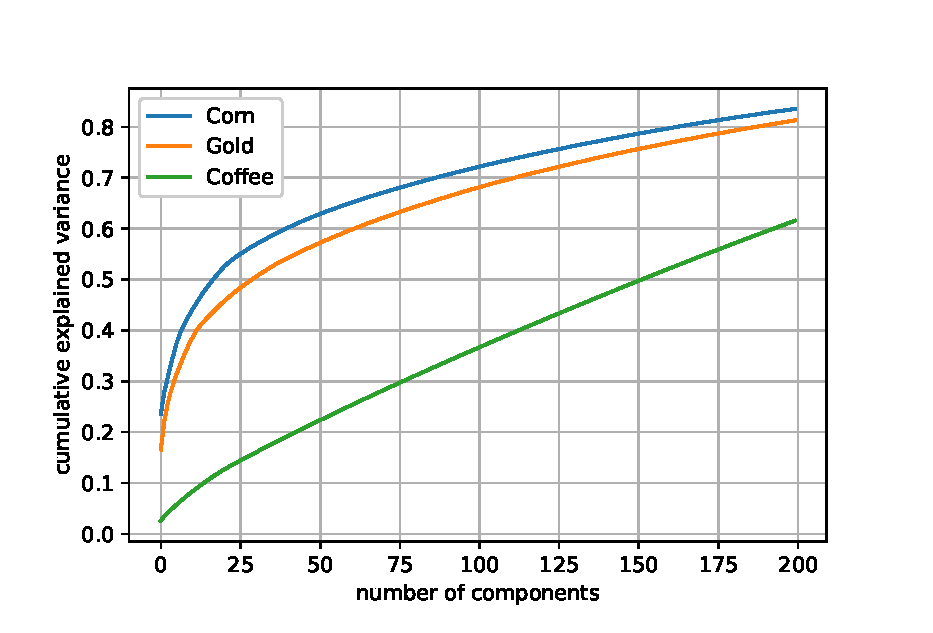
\includegraphics{figures/pca.eps}
    \caption{PCA explained variance}
\end{figure}

\subsection{Project Design}

Following schema is showing high level project pipeline.
\newline

\tikzstyle{block} = [draw, fill=blue!20, rectangle, 
    minimum height=3em, minimum width=6em]
\tikzstyle{sum} = [draw, fill=blue!20, circle, node distance=1cm]
\tikzstyle{input} = [coordinate]
\tikzstyle{output} = [coordinate]
\tikzstyle{pinstyle} = [pin edge={to-,thin,black}]

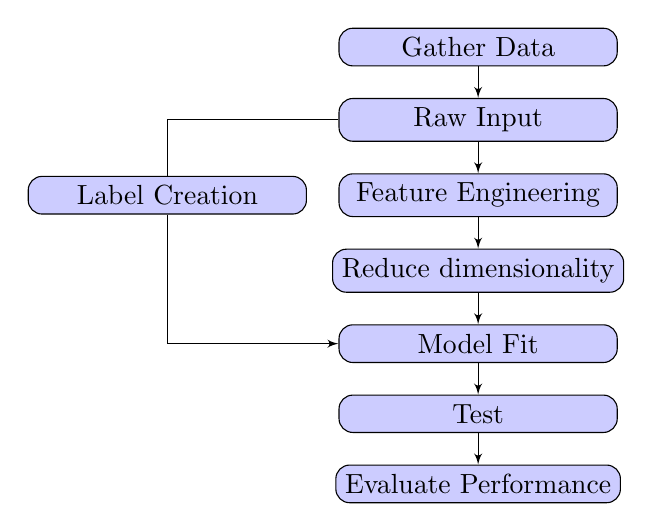
\begin{tikzpicture}[node distance=4mm, >=latex',
 block/.style = {draw, rectangle, minimum height=10mm, minimum width=28mm,align=center},
rblock/.style = {draw, rectangle, rounded corners=0.5em, fill=blue!20,
                 minimum width={width("Reduce dimensionality")+2pt}},
tblock/.style = {draw, trapezium, minimum height=10mm, 
                 trapezium left angle=75, trapezium right angle=105, align=center},
                        ]

    \node [rblock]                      (gd)      {Gather Data};
    \node [rblock, below=of gd]         (input)   {Raw Input};
    \node [rblock, below=of input]      (fe)      {Feature Engineering};
    \node [rblock, below=of fe]         (rd)      {Reduce dimensionality};
    \node [rblock, left=of fe]          (label)   {Label Creation};
    \node [rblock, below=of rd]         (mf)      {Model Fit};
    \node [rblock, below=of mf]         (tst)     {Test};
    \node [rblock, below=of tst]        (perf)    {Evaluate Performance};

    \path[draw,->] (gd)         edge (input)
                   (input)      edge (fe)
                   (fe)         edge (rd)
                   (rd)         edge (mf)
                   (input)      -|   (label)
                   (label)      |-   (mf)
                   (mf)         edge (tst)
                   (tst)        edge (perf)
                    ;
\end{tikzpicture}
\newline
\newline
I will look into commodities that's why I want to capture seasonality.
I plan to use daily data, because of that my trading plan is to hold the position (either long/short) for 1--3 days or until stop loss was hit.

I will investigate different features that have impact on trading.

\begin{itemize}
    \item feature engineering
    \begin{itemize}
        \item PCA (dimensionality of input vector is very high)
        \item COT
        \item price
        \item volume
        \item date (modify to find seasonality)
    \end{itemize}
    \item training
    \begin{itemize}
        \item Random Forest
        \item Neural Network
        \item XGBoost
        \item LightGBM
        \item \ldots
    \end{itemize}
\end{itemize}

How will be stop-loss selected?
\begin{itemize}
    \item fixed
        \begin{itemize}
            \item try different fixed stop-loss values
        \end{itemize}
    \item floating
        \begin{itemize}
            \item based on the volatility of previous days
        \end{itemize}
\end{itemize}

\subsection{Raw Input}
Raw input will have approximately following shape:
\[2 \textup{ years data}\]
\[2*252 \textup{ trading days} = 504\textup{ trading days}\]
\[504\textup{ trading days} * 7 \textup{ (number of features in a day)} = 3528 \textup{ features}\]

\subsection{Feature Engineering}
Reduce dimensionality:
\begin{itemize}
    \item PCA
    \item accumulation
        \begin{itemize}
            \item trading day of month
            \item average
            \item try different min/max of last trading day in relationship to 2years of data
            \item \ldots
        \end{itemize}
\end{itemize}

\subsection{Label Generation}
Labels will be generated as,
% \[
% \begin{align}
\begin{gather}
    fee = 1.5 \\
    t_{treshold} = 30 \\
    v_{volatility} = (\textup{close} - \textup{open})*\delta \textup{ where } \delta \approx 0.95 \\
    %\textup{label} = 
    labels
    \begin{cases}
        | v_{volatility} | > t_{treshold} + fee \implies
        \begin{cases}
            v_{volatility} > 0 \implies 1 \textup{ (long)} \\
            v_{volatility} < 0 \implies -1 \textup{ (short)} \\
        \end{cases}\\
        | v_{volatility} | < t_{treshold} + fee \implies 0 \textup{ (no trade)}
    \end{cases}
% \end{align}
\end{gather}
% \]
$\delta$ constant is used for simulating slippage.
$1.5$ that we are subtracting is a trading fee.
We can see in the label function if volatility is too close to $0$ it will be rounded to $0$ --- meaning don't trade.

Output of model will be classification of input into three categories trade (long/short position) or do not trade.

If we will look into longer trading than one day. Labels can be constructed in the similar way as above. But we will have to consider stop-loss value. We might have to end the trade sooner than we wanted.

\section{Benchmark Model}

I will use three benchmarks for my model

\begin{itemize}
    \item fixed percentage (bank/bond deposit comparison)
    \item Dow Jones Industrial Average performance
    \item mean reversal trading on given commodity markets
\end{itemize}

\section{Evaluation of trading}

Compare trading strategy to Nasdaq performance and mean reversal strategy.

\section{Conclusion}

Trading is a difficult ML problem. Out of three compared commodities gold, corn and coffee we were able to predict performance with gold. Other commodities behaved randomly with approximately 0 correlation to the actual volatility.

In the beginning of project, I was thinking of a classifier (short, no trade, long) because it is closer to the usage of model. I tested regressor as well. Regressor works better because there is more information. I tried different loss function when training regressor. I decided to use weighted MSE. This could be further modified for better function omitting errors below threshold.

Gold trading is the most capital intensive with very big stop losses (1000 long, 800 short). This can be problem for trading with $10 000\$$ account.

In case of corn and coffee the data was almost impossible to classify. I suspect more data transformation is needed to get better results.

\end{document}
